\subsubsection{Caso d'uso UC8.1.3.2: Creazione domanda a risposta multipla}
	\label{UC8.1.3.2}
	\begin{figure}[h]
		\centering
			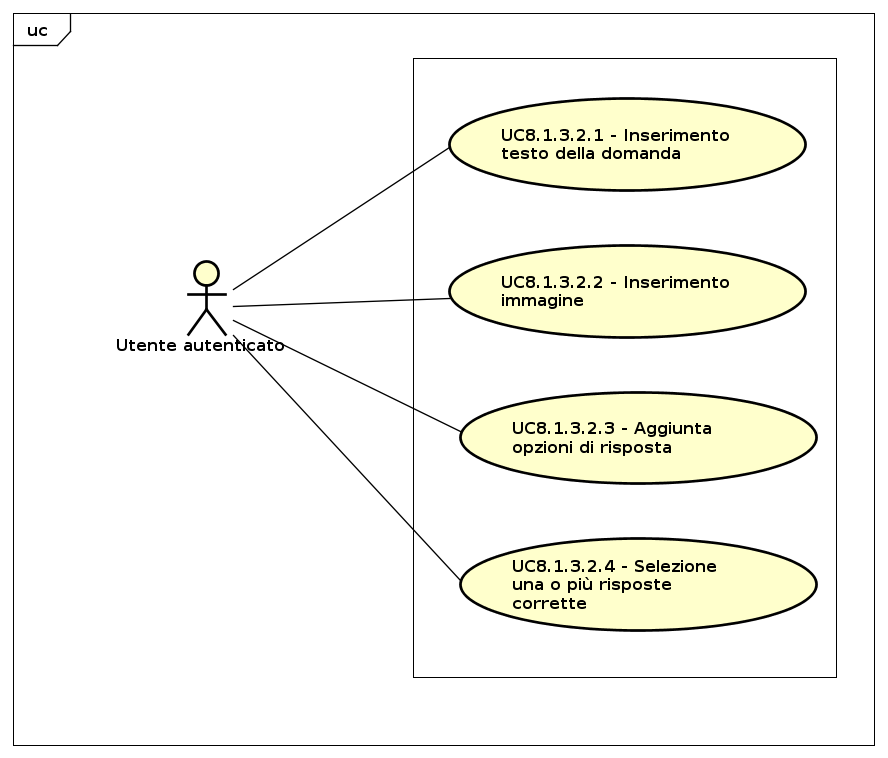
\includegraphics[scale=0.45,keepaspectratio]{UML/UC8_1_3_2.png}
		\caption{UC8.1.3.2: Creazione domanda a risposta multipla}
	\end{figure}
	\FloatBarrier
	\begin{itemize}
		\item
			\textbf{Attori}: utente autenticato, utente autenticato pro;
		\item		
			\textbf{Descrizione}: l'attore può utilizzare la procedura guidata per la creazione di una domanda a risposta multipla;
		\item
			\textbf{Precondizione}: l'attore ha selezionato la funzionalità di creazione di una domanda a risposta multipla;
		\item
			\textbf{Postcondizione}: l'attore ha creato una domanda a risposta multipla;
		\item
			\textbf{Scenario principale}:
	       		\begin{enumerate}
	       			\item
	       			L'attore può inserire il testo della domanda (UC8.1.3.2.1);
	       			\item
	       			L'attore può inserire un'immagine relativa al testo della domanda (UC8.1.3.2.2);
	       			\item
	       			L'attore può aggiungere almeno due opzioni di risposta (UC8.1.3.2.3);
					\item
					L'attore può indicare una o più risposte corrette (UC8.1.3.2.4).
	 			\end{enumerate}
	\end{itemize}

\subsubsection{Caso d'uso UC8.1.3.2.1: Inserimento testo della domanda}
	\begin{itemize}
		\item
			\textbf{Attori}: utente autenticato, utente autenticato pro;
		\item		
			\textbf{Descrizione}: l'attore può inserire il testo della domanda;
		\item
			\textbf{Precondizione}: l'attore ha selezionato la funzionalità di creazione di una domanda a risposta multipla; 
		\item
			\textbf{Postcondizione}: l'attore ha inserito il testo della domanda;
		\item
			\textbf{Scenario principale}: l'attore inserisce il testo della domanda. 
	 			
	\end{itemize}
	
\subsubsection{Caso d'uso UC8.1.3.2.2: Inserimento immagine}
	\label{UC8.1.3.2.2}
	\begin{figure}[h]
		\centering
			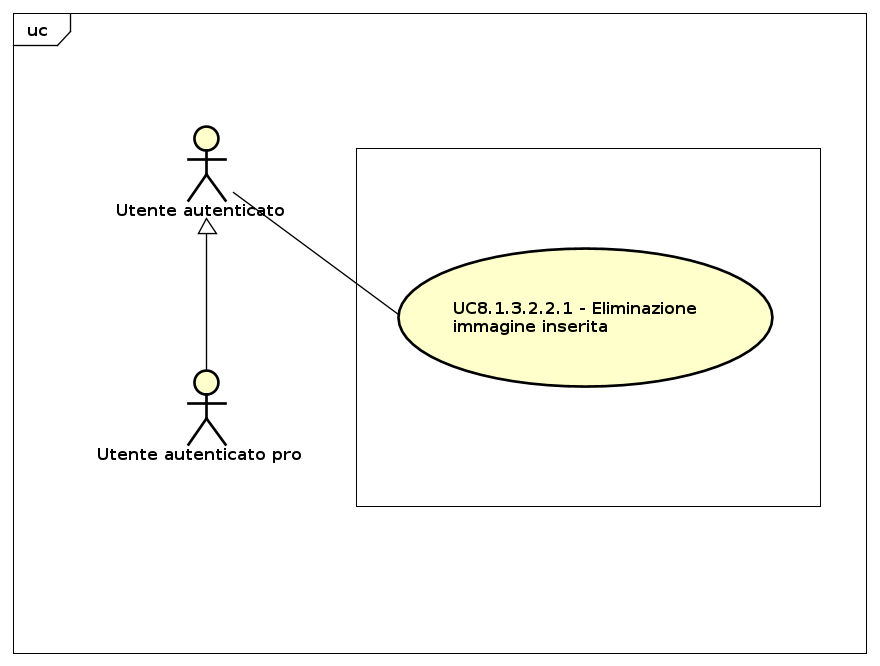
\includegraphics[scale=0.45,keepaspectratio]{UML/UC8_1_3_2_2.png}
		\caption{UC8.1.3.2.2: Inserimento immagine}
	\end{figure}
	\FloatBarrier
	\begin{itemize}
		\item
			\textbf{Attori}: utente autenticato, utente autenticato pro;
		\item		
			\textbf{Descrizione}: l'attore può inserire un'immagine relativa al testo della domanda;
		\item
			\textbf{Precondizione}: l'attore ha selezionato la funzionalità di creazione di una domanda a risposta multipla; 
		\item
			\textbf{Postcondizione}: l'attore ha inserito un'immagine relativa al testo della domanda;
		\item
			\textbf{Scenario principale}: 
			\begin{enumerate}
				\item
					L'attore può eliminare l'immagine inserita (UC8.1.3.2.2.1).	
			\end{enumerate}						
	\end{itemize}

\subsubsection{Caso d'uso UC8.1.3.2.2.1: Eliminazione immagine inserita}
		\begin{itemize}
		\item
			\textbf{Attori}: utente autenticato, utente autenticato pro;
		\item		
			\textbf{Descrizione}: l'attore può rimuovere l'immagine relativa al testo della domanda che era stata inserita precedentemente;
		\item
			\textbf{Precondizione}: l'attore ha inserito un immagine relativa al testo della domanda;
		\item
			\textbf{Postcondizione}: l'attore ha eliminato l'immagine relativa alla domanda;
		\item
			\textbf{Scenario principale}: l'attore rimuove l'immagine relativa alla domanda. 
		\end{itemize}
	
\subsubsection{Caso d'uso UC8.1.3.2.3: Aggiunta opzioni di risposta}
	\label{UC8.1.3.2.3}
	\begin{figure}[h]
		\centering
			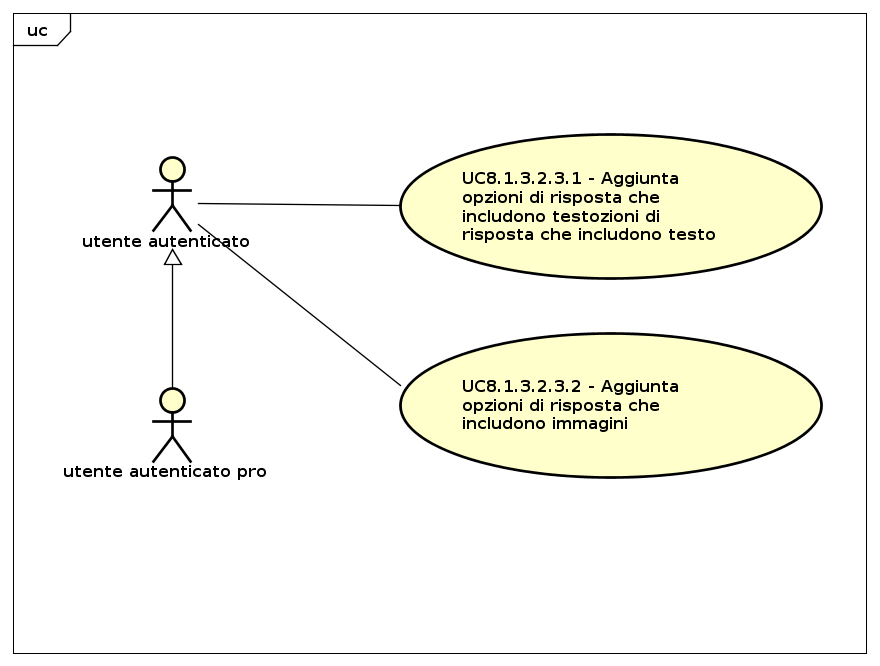
\includegraphics[scale=0.45,keepaspectratio]{UML/UC8_1_3_2_3.png}
		\caption{UC8.1.3.2.3: Aggiunta opzioni di risposta}
	\end{figure}
	\FloatBarrier
	\begin{itemize}
		\item
			\textbf{Attori}: utente autenticato, utente autenticato pro;
		\item		
			\textbf{Descrizione}: l'attore può aggiungere almeno due opzioni di risposta;
		\item
			\textbf{Precondizione}: l'attore ha selezionato la funzionalità di creazione di una domanda a risposta multipla;
		\item
			\textbf{Postcondizione}: l'attore ha aggiunto due o più opzioni di risposta;
		\item
			\textbf{Scenario principale}:
	       		\begin{enumerate}
	       			\item
	       			L'attore può aggiungere opzioni di risposta che includono testo (UC8.1.3.2.3.1);
					\item
					L'attore può aggiungere opzioni di risposta che includono immagini (UC8.1.3.2.3.2).
	 			\end{enumerate}
	\end{itemize}	

\subsubsection{Caso d'uso UC8.1.3.2.3.1: Aggiunta opzioni di risposta che includono testo}
	\label{UC8.1.3.2.3.1}
	\begin{figure}[h]
		\centering
			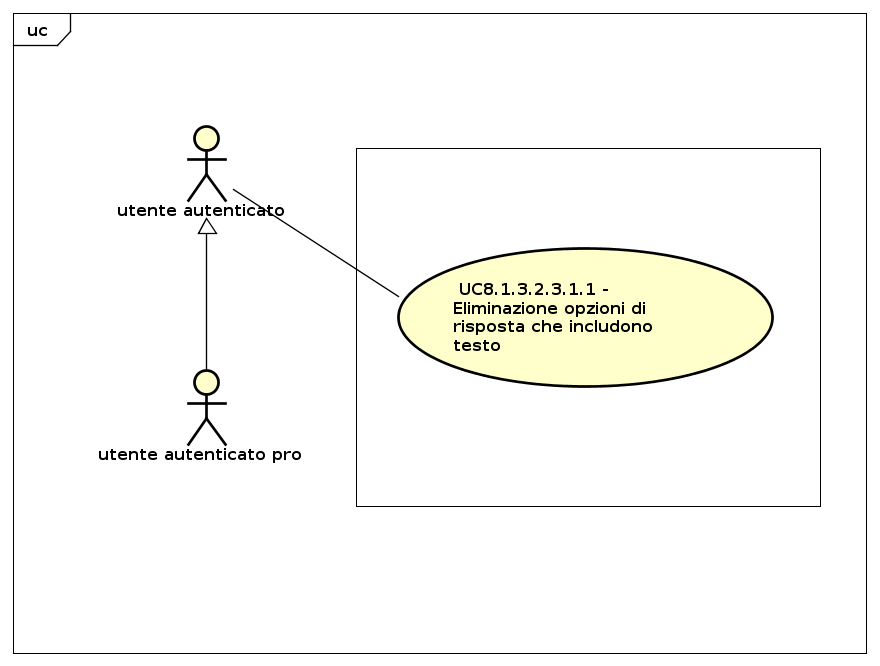
\includegraphics[scale=0.45,keepaspectratio]{UML/UC8_1_3_2_3_1.png}
		\caption{UC8.1.3.2.3.1: Aggiunta opzioni di risposta che includono testo}
	\end{figure}	
	\FloatBarrier
	\begin{itemize}
		\item
			\textbf{Attori}: utente autenticato, utente autenticato pro;
		\item		
			\textbf{Descrizione}: l'attore può aggiungere almeno due opzioni di risposta che includono testo;
		\item
			\textbf{Precondizione}: l'attore ha selezionato la funzionalità di creazione di una domanda a risposta multipla;
		\item
			\textbf{Postcondizione}: l'attore ha aggiunto due o più opzioni di risposta che includono testo;
		\item
			\textbf{Scenario principale}: 
				\begin{enumerate}
					\item
						L'attore può eliminare un'opzione che include testo (UC8.1.3.2.3.1.1).				
				\end{enumerate}
	\end{itemize}	
	
\subsubsection{Caso d'uso UC8.1.3.2.3.1.1: Eliminazione opzioni di risposta che includono testo}
		\begin{itemize}
		\item
			\textbf{Attori}: utente autenticato, utente autenticato pro;
		\item		
			\textbf{Descrizione}: l'attore può rimuovere un'opzione di risposta che include testo;
		\item
			\textbf{Precondizione}: l'attore ha inserito almeno un'opzione di risposta che include testo;
		\item
			\textbf{Postcondizione}: l'attore ha eliminato l'opzione di risposta che include testo;
		\item
			\textbf{Scenario principale}: l'attore rimuove un'opzione di risposta che include testo.				
		\end{itemize}

\subsubsection{Caso d'uso UC8.1.3.2.3.2: Aggiunta opzioni di risposta che includono immagini}
	\label{UC8.1.3.2.3.2}
	\begin{figure}[h]
		\centering
			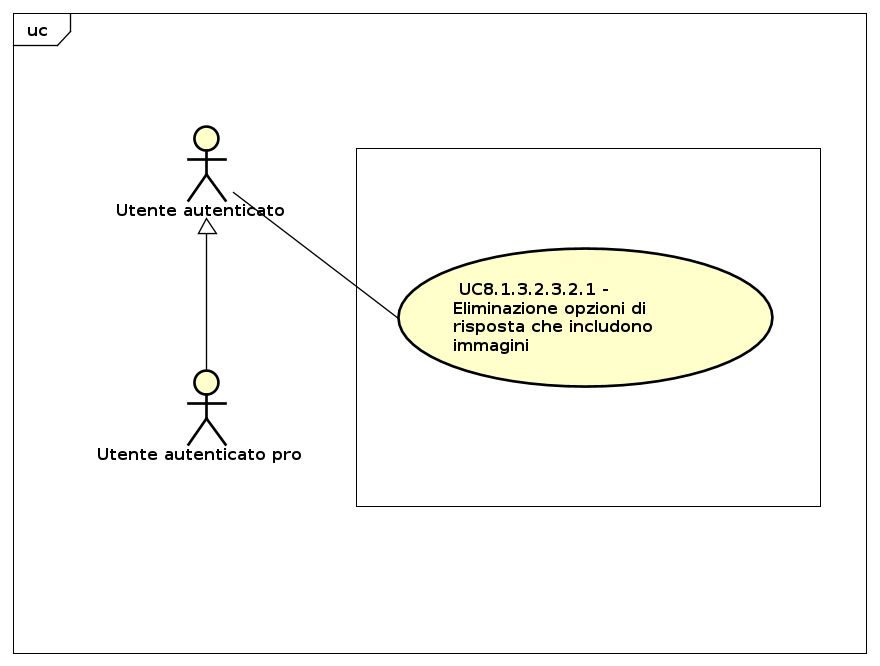
\includegraphics[scale=0.45,keepaspectratio]{UML/UC8_1_3_2_3_2.png}
		\caption{UC8.1.3.2.3.2:  Aggiunta opzioni di risposta che includono immagini}
	\end{figure}	
	\FloatBarrier
	\begin{itemize}
		\item
			\textbf{Attori}: utente autenticato, utente autenticato pro;
		\item		
			\textbf{Descrizione}: l'attore può aggiungere almeno due opzioni di risposta che includono immagini;
		\item
			\textbf{Precondizione}: l'attore ha selezionato la funzionalità di creazione di una domanda a risposta multipla;
		\item
			\textbf{Postcondizione}: l'attore ha aggiunto due o più opzioni di risposta che includono immagini;
		\item
			\textbf{Scenario principale}: 
				\begin{enumerate}
					\item
						L'attore può eliminare un'opzione che include un'immagine (UC8.1.3.2.3.2.1); 				
				\end{enumerate}
	\end{itemize}
	
\subsubsection{Caso d'uso UC8.1.3.2.3.2.1: Eliminazione opzioni di risposta che includono immagini}
		\begin{itemize}
		\item
			\textbf{Attori}: utente autenticato, utente autenticato pro;
		\item		
			\textbf{Descrizione}: l'attore può rimuovere un'opzione di risposta che include un'immagine;
		\item
			\textbf{Precondizione}: l'attore ha inserito almeno un'opzione di risposta che include un'immagine;
		\item
			\textbf{Postcondizione}: l'attore ha eliminato l'opzione di risposta che include un'immagine;
		\item
			\textbf{Scenario principale}: l'attore rimuove un'opzione di risposta che include un'immagine.				
		\end{itemize}
		
\subsubsection{Caso d'uso UC8.1.3.2.4: Selezione una o più risposte corrette}
	\begin{itemize}
		\item
			\textbf{Attori}: utente autenticato, utente autenticato pro;
		\item		
			\textbf{Descrizione}: l'attore può indicare una o più risposte corrette;
		\item
			\textbf{Precondizione}: l'attore ha selezionato la funzionalità di creazione di una domanda a risposta multipla;
		\item
			\textbf{Postcondizione}: l'attore ha selezionato una o più risposte corrette;
		\item
			\textbf{Scenario principale}: l'attore indica una o più risposte corrette. 			
	\end{itemize}